\section{Experimental Design}
\label{sec:expdesign}

\subsection{Introduction}
\begin{frame}
  \frametitle{Research Overview}
  \begin{minipage}{0.5\textwidth}
    How does the ability to determine forensic-relevant spent nuclear fuel
    attributes using machine learning techniques degrade as less information is
    available?
    \vspace*{2cm}
  \end{minipage}%
  \begin{minipage}{0.5\textwidth}
    \begin{figure}
      \centering
      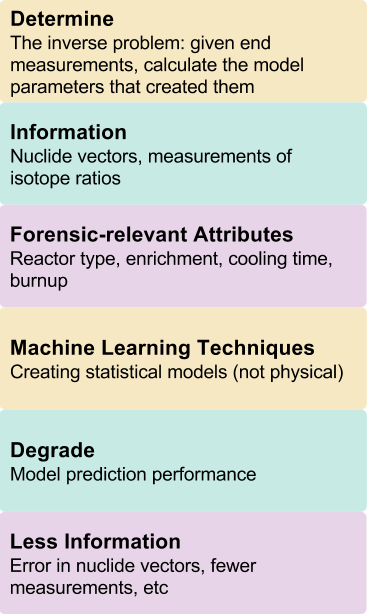
\includegraphics[height=0.75\textheight]{./figures/overview.png}
      \caption{Definitions of terms within the main research question}
    \end{figure}
  \end{minipage}
\end{frame}


\subsection{Algorithm Evaluation}

Additionally, machine learning algorithms are heavily dependent on the inputs
and parameters given to them, such as training set sizes, learning rates,
regularization, etc. To evaluate the performance or tweak the model from an
algorithm, diagnostic plots will be used. Learning and validation curves will
indicate how the models are performing, initially both with respect to the
testing error and the cross validation error. As previously mentioned, these
two errors are to be compared to the training error to understand the
prediction and generalization strength with respect to training set size and
the algorithm parameters governing model complexity. 

The learning curves were obtained as follows. For a given (randomly chosen)
training set size between 15 and 100\% of the total data set, several training
and prediction rounds were performed. The repetition for obtaining the testing
error is the same value as the \textit{k} in k-fold cross validation. The
testing error scenario averages the values of the obtained errors whereas the
k-fold cross-validation performs this automatically.  The validation curves
were obtained as follows. For a given parameter, the value of the parameter is
varied and \textit{k} training and prediction phases are completed, and their
errors averaged. Again, for k-fold cross-validation, these errors are already
averaged. The learning curves help determine if we are over- or under-training.
The validation curves help determine the optimal way to be robust to over- and
under-fitting. 

% confidence interval stuff for future paper
%2. Regression Training Error: Confidence intervals on predictions to understand
%true error versus sample error Test set must be > 30 instances, Can easily
%calculate N\% confidence interval.
%2. redo confidence interval study


\subsection{Comparing Algorithms}

Maybe can delete this if I already discuss it in the above section. Options for
comparison of algorithms: Comparing classification of 2 classes on same ROC
plot with multiple ML systems, Scatter plots, Pairwise t-tests. 

\section{Posting here for now}

1. Learning curve
2. Validation curve
3. Random error curve

Want to show the difference between test/train error plots and CV/train error
plots.  Determine some argument that perfers the latter. For the above
categories in the validation section, can show plots directly next to each
other (for 1, 2, 3) to hopefully show that cross validation provides better
generalizability.

\todo{Discuss understanding confidence intervals in predictions.}

%\input{./chapters/methodology/experiment/other_stuff}
